\documentclass[border=12pt]{standalone}
\usepackage{tikz}
\usetikzlibrary{positioning, calc, fit, backgrounds, arrows.meta}
\usepackage{amsmath, amssymb}

\begin{document}
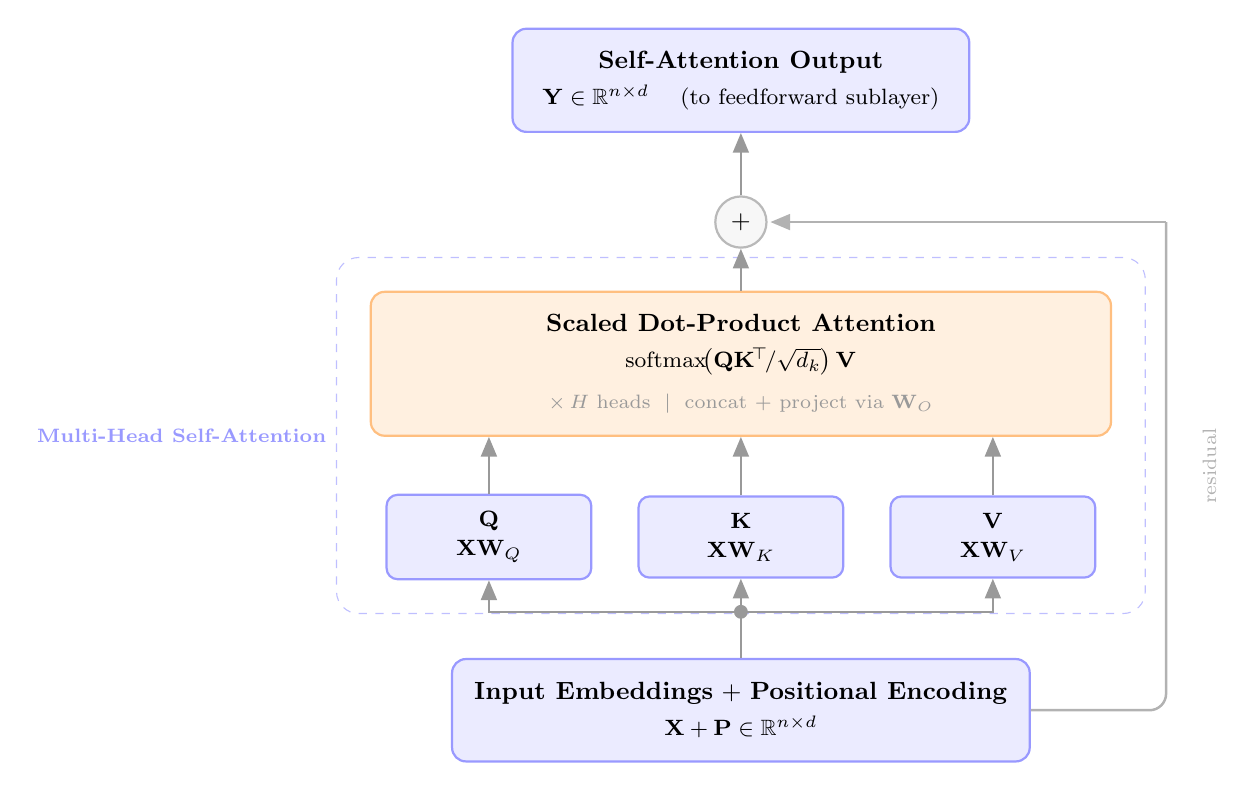
\begin{tikzpicture}[
    block/.style = {rectangle, draw=gray!60, thick, rounded corners=5pt,
                    minimum height=1.3cm, minimum width=5.8cm,
                    font=\small, inner sep=8pt, align=center},
    smallblock/.style = {rectangle, draw=gray!50, thick, rounded corners=4pt,
                    minimum height=1.0cm, minimum width=2.6cm,
                    font=\footnotesize, inner sep=6pt, align=center},
    arr/.style   = {line width=0.9pt, draw=black!40,
                    -{Triangle[length=2.5mm, width=2mm, fill=black!40]}},
    plainline/.style = {line width=0.9pt, draw=black!40},
    resline/.style = {line width=0.9pt, draw=black!30, rounded corners=6pt},
    resarr/.style  = {line width=0.9pt, draw=black!30,
                      -{Triangle[length=2.5mm, width=2mm, fill=black!30]}},
    plus/.style  = {circle, draw=gray!55, thick, fill=gray!6,
                    minimum size=0.65cm, font=\small, inner sep=0pt},
    lbl/.style   = {font=\footnotesize, text=black!50, align=center},
]

%% ---- Layout coordinates ----
\def\yInput{0}
\def\yQKV{2.2}
\def\yAttn{4.4}
\def\yAddA{6.2}
\def\yOut{8.0}
\def\resoff{5.4}

%% ==================================================================
%% NODES
%% ==================================================================

\node[block, fill=blue!8, draw=blue!40] (input) at (0, \yInput)
    {\textbf{Input Embeddings} + \textbf{Positional Encoding}\\[2pt]
     {\footnotesize $\mathbf{X} + \mathbf{P}\in\mathbb{R}^{n\times d}$}};

\node[smallblock, fill=blue!8, draw=blue!40] (wq) at (-3.2, \yQKV)
    {\textbf{Q}\\[1pt]$\mathbf{X}\mathbf{W}_{Q}$};
\node[smallblock, fill=blue!8, draw=blue!40] (wk) at (0, \yQKV)
    {\textbf{K}\\[1pt]$\mathbf{X}\mathbf{W}_{K}$};
\node[smallblock, fill=blue!8, draw=blue!40] (wv) at (3.2, \yQKV)
    {\textbf{V}\\[1pt]$\mathbf{X}\mathbf{W}_{V}$};

\node[block, fill=orange!12, draw=orange!50, minimum width=9.4cm] (attn)
    at (0, \yAttn)
    {\textbf{Scaled Dot-Product Attention}\\[2pt]
     {\footnotesize $\operatorname{softmax}\!\bigl(\mathbf{Q}\mathbf{K}^{\!\top}
      \!/\sqrt{d_{k}}\bigr)\,\mathbf{V}$}\\[4pt]
     {\scriptsize\color{black!40} $\times\,H$ heads $\;\vert\;$
      concat + project via $\mathbf{W}_{O}$}};

\node[plus] (add1) at (0, \yAddA) {$+$};

\node[block, fill=blue!8, draw=blue!40] (output) at (0, \yOut)
    {\textbf{Self-Attention Output}\\[2pt]
     {\footnotesize $\mathbf{Y}\in\mathbb{R}^{n\times d}$
      \quad (to feedforward sublayer)}};

%% ==================================================================
%% CONNECTIONS
%% ==================================================================

%% Fan-out: Input -> Q, K, V
\coordinate (branch) at (0, {0.5*(\yInput + \yQKV) + 0.15});
\draw[plainline] (input.north) -- (branch);
\fill[black!40] (branch) circle (2.5pt);
\draw[arr] (branch) -| (wq.south);
\draw[arr] (branch) -- (wk.south);
\draw[arr] (branch) -| (wv.south);

%% Q, K, V -> Attention
\draw[arr] (wq.north) -- (wq.north |- attn.south);
\draw[arr] (wk.north) -- (attn.south);
\draw[arr] (wv.north) -- (wv.north |- attn.south);

%% Attention -> Add1
\draw[arr] (attn.north) -- (add1.south);

%% Add1 -> Output
\draw[arr] (add1.north) -- (output.south);

%% Residual: Input east -> up right side -> left into Add1
\draw[resline] (input.east) -- (\resoff, \yInput)
    -- (\resoff, \yAddA);
\draw[resarr, shorten >=1pt] (\resoff, \yAddA) -- (add1.east);
\node[lbl, font=\scriptsize, text=black!30]
    at (\resoff + 0.55, {0.5*(\yInput + \yAddA)})
    {\rotatebox{90}{residual}};

%% ==================================================================
%% GROUPING BOX
%% ==================================================================
\begin{scope}[on background layer]
    \node[draw=blue!25, dashed, rounded corners=8pt, inner sep=12pt,
          fit=(wq)(wk)(wv)(attn),
          label={[font=\scriptsize\bfseries, blue!40]left:%
                 Multi-Head Self-Attention}] (mhabox) {};
\end{scope}

\end{tikzpicture}
\end{document}
